\documentclass[12pt,letter]{article}
\usepackage[moduleName={Super Echo}]{KautenjaDSP}
\begin{document}
\titlePage{img/Logo}{img/Module}{img/KautenjaDSP}

% -------------------
% MARK: Overview
% -------------------

\section{Overview}

Super Echo is a Eurorack module that emulates the echo effect from the S-SMP sound chip on the Super Nintendo Entertainment System (SNES). The Echo effect of the S-SMP chip has $15$ different delay levels of $16ms$ each, a $64KB$ echo buffer, an 8-tap FIR filter for shaping the sound of the echo, parameterized feedback, and parameterized dry / wet mix level. The echo buffer is stereo, although the echo parameters and coefficients of the FIR filter are the same for both channels. Super Echo provides the key features of the echo module of the S-SMP chip, namely,
\begin{itemize}
  \item \textbf{Stereo Processing:} Dual echo buffers for two independent inputs in stereo configuration.
  \item \textbf{Expanded Delay:} The 15 levels of delay has been upgraded to 31 levels that each add an additional $16ms$ of delay (up to roughly $500ms$).
  \item \textbf{Feedback:} Additive and subtractive feedback following the original implementation
  \item \textbf{8-tap FIR Filter:} Fully parameterized 8-tap FIR filter for shaping the sound of the echo. The filter can be parameterized as low-pass, high-pass, band-pass, band-stop, etc. and includes presets with filter parameters from popular SNES games.
\end{itemize}

\begin{figure}[!b]
\centering
\includegraphics[width=0.5\textwidth]{img/Chip}
\caption{\small The S-SMP module from the SNES. The S-SMP included two discrete microprocessors: the SPC700, and the S-DSP. The SPC700 performed primary computation, while the S-DSP performed DSP specific computations, like BRR decoding, sample playback, applying the echo effect, mixing levels, etc. The SPC700 and S-DSP shared $64KB$ of total RAM that was used for BRR sample data and the echo buffer. The digital audio is decoded back to an analog signal by a 16-bit DAC and amplified using an Op-Amp. Before digital-to-analog conversion, the output audio is low-pass filtered by a Gaussian filter that gives the S-SMP chip a distinctive sound.}
\end{figure}

% -------------------
% MARK: Panel Layout
% -------------------

\clearpage
\section{Panel Layout}

\begin{figure}[!htp]
\centering
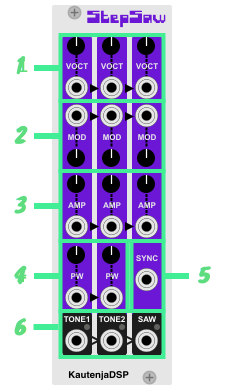
\includegraphics{img/Interface}
\end{figure}

\clearpage
\begin{enumerate}
  \item TODO
\end{enumerate}

\end{document}
